\documentclass[12pt]{article}

\usepackage[german]{babel}
\usepackage{amsmath}
\usepackage{amssymb} % to display symbols for real numbers, integers etc. Usage: \mathbb{R}
\usepackage{graphicx}
\usepackage{listings} % to display programming code
%\usepackage[ngerman]{babel}
\usepackage{color}
\usepackage{relsize} % to display scaled math symbols (big summation symbol etc.)
\usepackage{textcomp}

\DeclareGraphicsExtensions{.pdf,.jpeg,.png}
\definecolor{listinggray}{gray}{0.9}
\definecolor{lbcolor}{rgb}{0.9,0.9,0.9}
\lstset{ % to display programming code in nice colors
	backgroundcolor=\color{lbcolor},
	tabsize=4,
	rulecolor=,
	language=matlab,
		basicstyle=\scriptsize, %for extra small font size
        upquote=true,
        aboveskip={1.5\baselineskip},
        columns=fixed,
        showstringspaces=false,
        extendedchars=true,
        breaklines=true,
        prebreak = \raisebox{0ex}[0ex][0ex]{\ensuremath{\hookleftarrow}},
		frame=single, %draw frame
        showtabs=false,
        showspaces=false,
        showstringspaces=false,
        identifierstyle=\ttfamily,
        keywordstyle=\color[rgb]{0,0,1},
        commentstyle=\color[rgb]{0.133,0.545,0.133},
        stringstyle=\color[rgb]{0.627,0.126,0.941},
        numbers=left,
        stepnumber=1,
        firstnumber=1,
        numberfirstline=true,
        linewidth=14cm,
}

\title{Uebungsblatt 4\\ \glqq Mustererkennung\grqq}
\author{J. Cavojska, N. Lehmann, R. Toudic}
\date{01.06.2015}
\begin{document}
\maketitle
%\renewcommand{\contentsname}{Table of Contents}
\tableofcontents
\newpage

\section{Aufbereitung der Daten}
\begin{lstlisting}[language=Matlab]
% fish.txt: index; the age of the fish; the water temperature in Celsius; the length of the fish
A = load('fish.txt');

% winequality-red.txt: fixed acidity; volatile acidity; citric acid; residual sugar; chlorides; free sulfur dioxide; total sulfur; dioxide; density; pH; sulphates; alcohol; quality (score between 0 and 10) 
B = load('winequality-red.txt');
\end{lstlisting}
\newpage

\section{Aufgabe 1 (Lineare Regression)}
\textit{Schaetzen Sie den Wert fuer length anhand der Parameter age und temperature mit linearer Regression.\\
Visualisieren Sie dreidimensional die tatsaechlichen Datenpunkte, die geschaetzten Datenpunkte, die Ebene auf die projiziert wurde, sowie die Abstaende der tatsaechlichen Datenpunkte zu dieser Ebene.}

\begin{lstlisting}[language=Matlab]
y = A(:,4);  % nur die Laengen der Fische
Z = A(:,2:3);  % alle Datenpunkte, ausser Laenge
onesVector = ones(size(Z,1), 1); % Spaltenvektor mit Einsen der gleichen Laenge wie A
X = horzcat(onesVector, Z);  % Einsen-Vektor an Datenpunkte-Matrix drankleben

% X' ist die transponierte Matrix X
beta = inv(X'*X) * X' * y;  % beta ist der Vektor, mit dem Eingabedaten multipliziert werden muessen, damit wir an die Klassen-Labels kommen
% Resultat:
% beta =
%     1.0e+03 *
%  
%      3.9043
%      0.0262
%     -0.1064

% Plot
figure('NumberTitle','off','Name','Aufgabe 1 - Mesh');
hold on

% Bildpunkte der Rohdaten
Bildpunkte = A(:,2:4);
scatter3(Bildpunkte(:,1), Bildpunkte(:,2), Bildpunkte(:,3),30,[0 0 1]);

% Bildpunkte der geschaetzten Daten
EstimatedLength = X*beta;
% Ebene mit Geschaetzter Laenge
EstimatedData = horzcat(Z, EstimatedLength);
% Plot
scatter3(EstimatedData(:,1), EstimatedData(:,2), EstimatedData(:,3),30,[0 1 0], 'filled');

% Intervalle bestimmen
min_A = min(A(:,2:4));
max_A = max(A(:,2:4));

x1 = min_A(1,1):5:max_A(1,1);
x2 = min_A(1,2):2:max_A(1,2);
[D1, D2] = meshgrid(x1,x2);
M = beta(1)+beta(2)*D1+beta(3)*D2;
surf(D1,D2,M);
colormap autumn;

% Linien von Datenpunkten auf Ebene einzeichnen
for index = 1:length(A(:,4))
     plot3([Z(index,1) Z(index,1)]',[Z(index,2) Z(index,2)]',[y(index) EstimatedLength(index)]','-b');
end

xlabel('Alter'); 
ylabel('Wassertemperatur'); 
zlabel('Laenge');
legend('Datenpunkte', 'regressierte Datenpunkte', 'regressierte Ebene')
\end{lstlisting}
Eine grafische Darstellung der tatsaechlichen und der durch die Regression entstandenen Datenpunkte:\\
\\
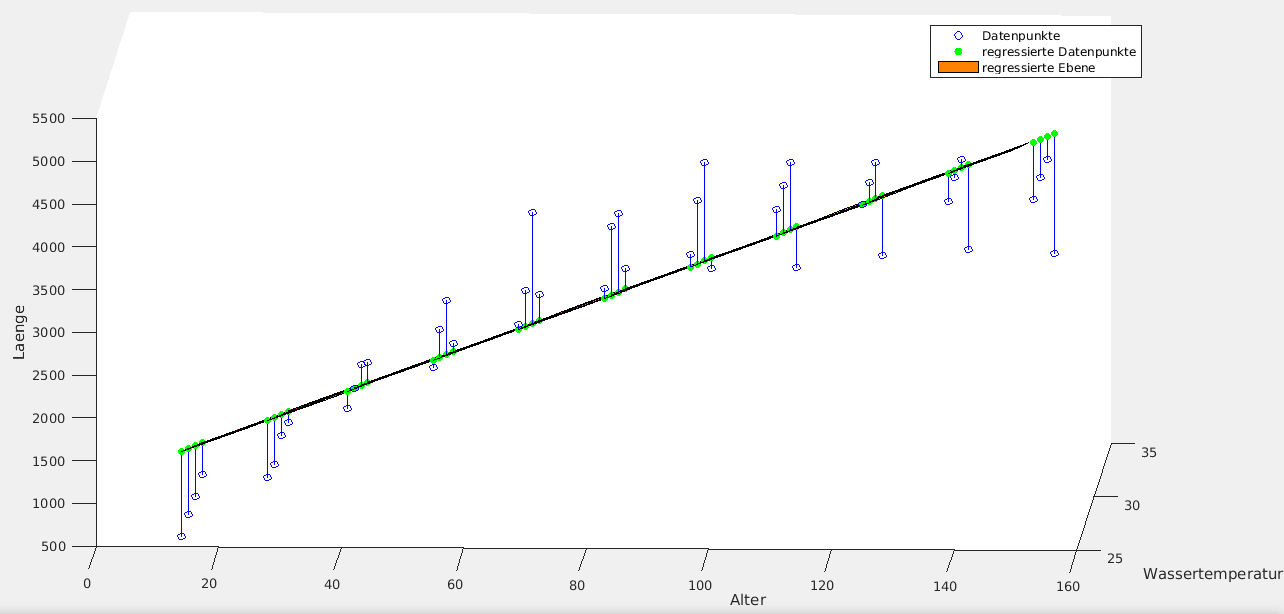
\includegraphics[width=14cm]{aufg1_ebene01.png}\\
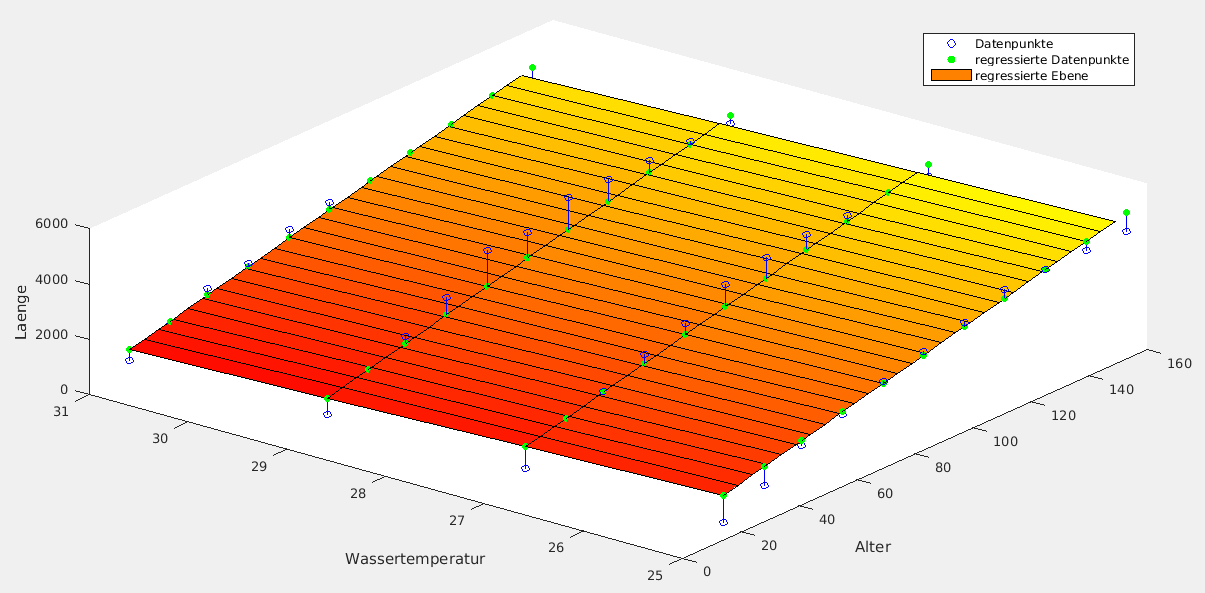
\includegraphics[width=14cm]{aufg1_ebene02.png}
\newpage

\section{Aufgabe 2 (Subset Selection)}
\textit{Schaetzen Sie den Wert fuer quality mit linearer Regression anhand aller moeglichen Kombinationen der anderen Parameter (also jeweils fuer alle Einer-­, Zweier-­, Dreierkombinationen, usw.) und berechnen jeweils die Summe der quadratischen Abweichungen zwischen den geschaetzten und tatsaechlichen Werten fuer quality.\\
Visualisieren Sie dies als zweidimensionalen Plot. Auf der x-Achse steht dabei die Anzahl der verwendeten Parameter, auf der y-­Achse die Summe der quadratischen Abweichungen.}
\begin{lstlisting}[language=Matlab]
y = B(:,12);  % Spalte mit Weinqualitaet
Result = [];  % Ergebnismatrix

featureIndices = [1 2 3 4 5 6 7 8 9 10 11];
for numFeatures = 1:11  % es gibt 11 features, anhand welcher man klassifizieren kann
    combinations = combnk(featureIndices, numFeatures); % combnk gibt eine Liste aller n ueber k vielen Kombinationen von featureIndices zurueck (wobei numFeatures unser k ist)
    for line = 1:size(combinations, 1)
        combination = combinations(line,:);
        X = B(:, combination);
        onesVector = ones(size(X,1), 1); % Spaltenvektor mit Einsen der gleichen Laenge wie B
        X = horzcat(onesVector, X);      % Einsen-Vektor an Datenpunkte-Matrix drankleben
        beta = inv(X'*X) * X' * y;       % beta ist der Vektor mit den Koeffizienten der Regressionsebene
        
        Q = (y - X*beta)'*(y - X*beta);  % mean squared error
        Result = vertcat(Result, [numFeatures, Q]);
    end
end % for numFeatures

figure('NumberTitle','off','Name','Aufgabe 2 - Scatter');
scatter(Result(:,1),Result(:,2));
\end{lstlisting}
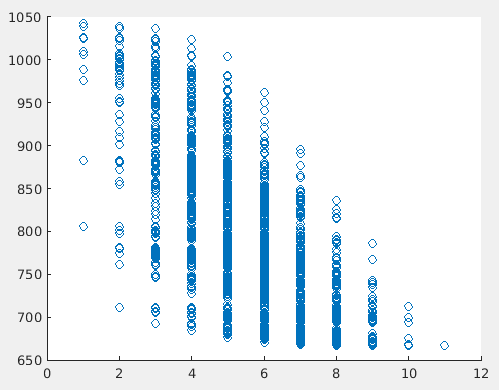
\includegraphics[width=10cm]{aufg2_subset_selection.png}

\end{document}